subsection{Bestimmung der Flächenträgheitsmomente}
Das Flächenträgheitsmoment ist eine Größe, die im weiteren Verlauf wichtig ist, um das Elastizitätsmodul der Stäbe zu ermitteln.
Es hängt von dem Querschnitt des Stabes, genauer der Abstände $y$ der Flächenelemente d$q$ zur neutralen Faser ab
\begin{equation}
I = \int_{Q} y ^2 \, \text{d}q \quad .
\end{equation}
Für den eckigen Stab benötigt man eine Formal für quadratische Quarschnitte. Die Kantenlänge sei $h$. Für $I_\text{E}$ gilt:
\begin{equation}
I_\text{E} = \int_{-\frac{h}{2}}^{\frac{h}{2}} \int_{-\frac{h}{2}}^{\frac{h}{2}} y^2\,  \text{d}x \text{d}y = \frac{1}{12} \cdot h^4 \quad .
\end{equation}
Um das Flächenträgheitsmoment für runde Querschnitte mit Radius $r$ zu berechnen, bietet sich die Verwendung von Polarkoordinaten an. Der Abstand zur $y$-Achse ist dann $r^2 \cdot \sin^2(x)$.  Mit der Jakobideterminante $r$ ist $I_R$
\begin{equation}
I_\text{R} = \int_{0}^{r}  \int_{0}^{2\pi} r^2 \cdot \sin^2(x) \cdot r  \, \text{d}\phi \text{d}r = \frac{1}{12}\cdot \pi \cdot r^4 \quad .
\end{equation}
Sowohl $h$ in wie auch der Durchmesser $2 \cdot r$ wurden sehr genau mit einer Schieblehre gemessen. Zu dem Fehler des Mittelwertes kommt allerdings eine Ableseungenauigkeit von \SI{0.05}{\milli\metre}  hinzu.

\begin{center}
	\captionof{table}{Breite $h$ des eckigen Stabes und Durchmesser $2 \cdot r$ des Runden}
\begin{tabular}{c|c}
	Breite $h$ in \SI{}{\milli\metre}& Durchmesser $2 \cdot r$ in \SI{}{\milli\metre}	\\
	\hline
	10.00 & 10.00 \\
	10.00  & 10.00 \\
	10.00  & 10.00 \\
	10.00  & 9.90 \\
	10.00  & 9.90 \\
	10.00  & 9.95 \\
	10.00  & 10.00 \\
	10.00  & 9.90 \\
	10.00  & 9.90 \\
	10.00 & 9.95 \\
\end{tabular}	
\end{center}

Für den eckigen Stab folgt aus dem Mittelwert der Breite
\begin{align}
  h = \SI{0.01000 \pm 0.00005}{\metre}
\end{align}
ein Flächenträgheitsmoment von
\begin{align}
I_\text{E}=\SI{3.88(17)e-10}{\metre\raiseto{4}} \quad .
\label{I_E}
\end{align}

Für den runden Stab folgt aus einem Radius von duschnittlich
\begin{equation}
  r = \SI{0.004975 \pm 0.000032}{\metre}
\end{equation}
das Flächenträgheitsmoment
\begin{equation}
  I_\text{R} = \SI{4.81(12)e-10}{\metre\raiseto{4}} \quad .
  \label{I_R}
\end{equation}


\subsection{Bestimmung des Elastizitätsmodul durch lineare Regression}
\subsubsection{Runder Stab -- einseitige Einspannung}
Die gemessene Durchbiegung $D(x)$ des Stabes wird durch die Gleichung \eqref{einseitige Einspannung} beschrieben.
Alle in ihr vorkommende Größen, bis auf das Elaatizitästmodul sind bekannt. Das Flächenträgheitsmoment wurde im vorherigen Abschnitt als \eqref{I_R} bestimmt und die herabziehende Kraft $F$ ist aus der Masse des Probekörpers zu berechnen
\begin{equation}
  F = m \cdot g = \SI{0.7476}{\kilo\gram} \cdot \SI{9.81}{\metre\per\second\squared} = \SI{7.3339}{\newton} \quad .
\end{equation}
Nun lässt sich das Elastizitäsmodul $E$ druch eine lineare Regression der Form
\begin{equation}
  D(x) = \frac{F}{2\cdot E I}\left(Lx^2-\frac{x^3}{3}\right) = \frac{1}{E} \cdot A +b
\end{equation}
bestimmen, indem $D(x)$ über $A$ ausgetragen wird (siehe Abbildung \ref{fig:Regression_runder_Stab}). $E$ entspricht dem Kehrwert der Steigung der Regressionsgeraden. Unter Verwendung der Formeln aus Kapitel~\ref{sec:regression} ergibt die Steigung mit Abweichung
\begin{equation}
  \frac{1}{E}= \SI{188.9(15)e-13}{\metre\squared\per\newton}
\end{equation}
und der $y$-Achsenabschnitt mit Abweichung
\begin{equation}
  b = \SI{14.33(36)e-05}{\metre} \quad.
\end{equation}
Das hier bestimmte Elastizitästmodul für den runden Stab ist folglich
\begin{equation}
  E = \SI{5.29(4)e+10}{\newton\per\metre\squared} \quad.
\end{equation}

\begin{figure}
\centering
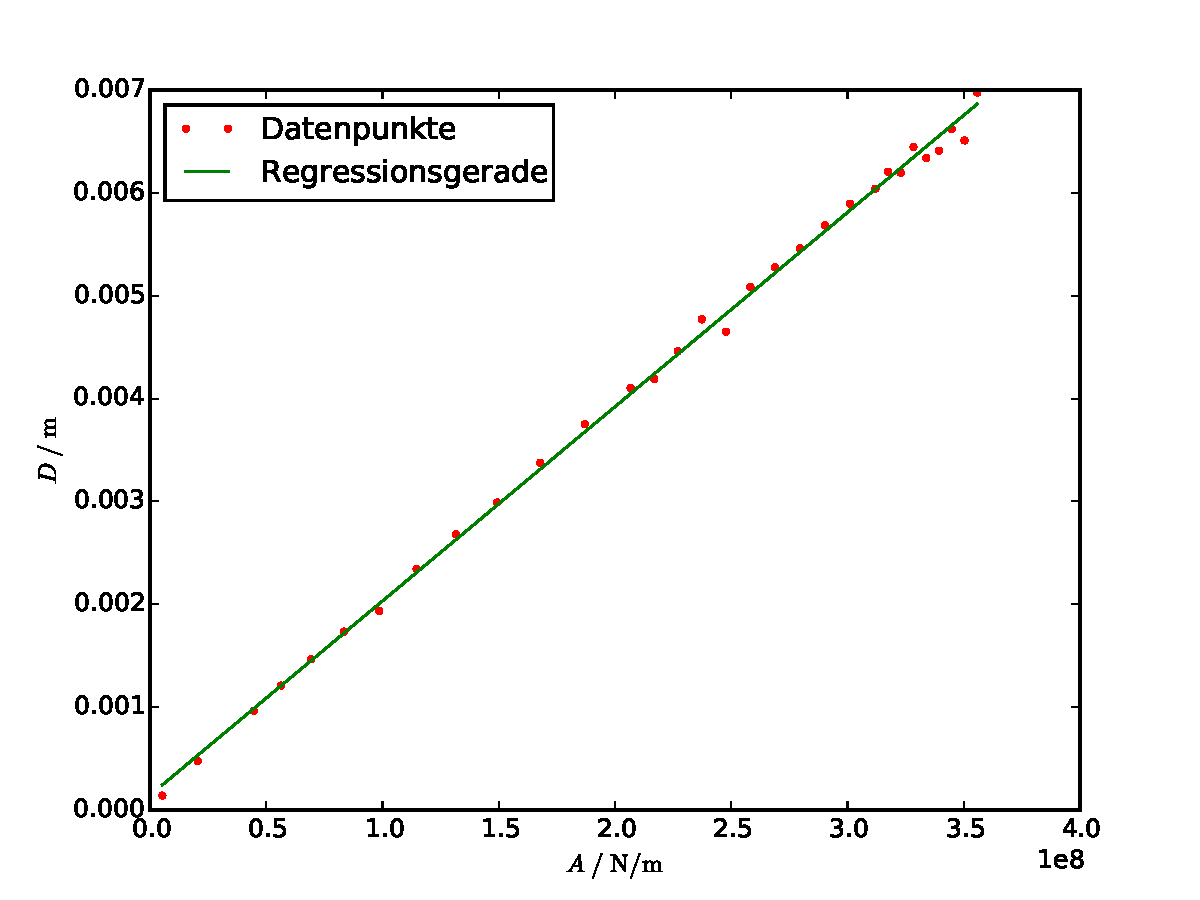
\includegraphics[width=\textwidth]{Regression_runder_Stab.pdf}
\caption{Regressionsgerade des runden Stabes bei einseitiger Einspannung}
\label{fig:Regression_runder_Stab}
\end{figure}



\subsubsection{Eckiger Stab -- einseitige Einspannung}
Hier ist der Vorgehensweise genau so, wie bei dem runden Stab. Es muss lediglich ein anderes Flächenträgheitsmoment \ref{I_E} und eine andere Kraft
\begin{equation}
  F = m \cdot g = \SI{0.7676}{\kilo\gram} \cdot \SI{9.81}{\metre\per\second\squared} = \SI{7.5302}{\newton}
\end{equation}
eingesetzt werden.
Dies führt auf eine Steigung mit Abweichung von
\begin{equation}
  \frac{1}{E}= \SI{135.6(9)e-13}{\metre\squared\per\newton}
\end{equation}
und den $y$-Achsenabschnitt mit Abweichung
\begin{equation}
  b = \SI{6.28(217)e-05}{\metre} \quad.
\end{equation}
Das hier bestimmte Elastizitästmodul für den eckigen Stab ist folglich
\begin{equation}
  E = \SI{7.37(5)e+10}{\newton\per\metre\squared} \quad.
\end{equation}
Die Werte wurden in Abbildung~\ref{fig:Regression_eckiger_Stab} aufgetragen.

\begin{figure}[h!]
\centering
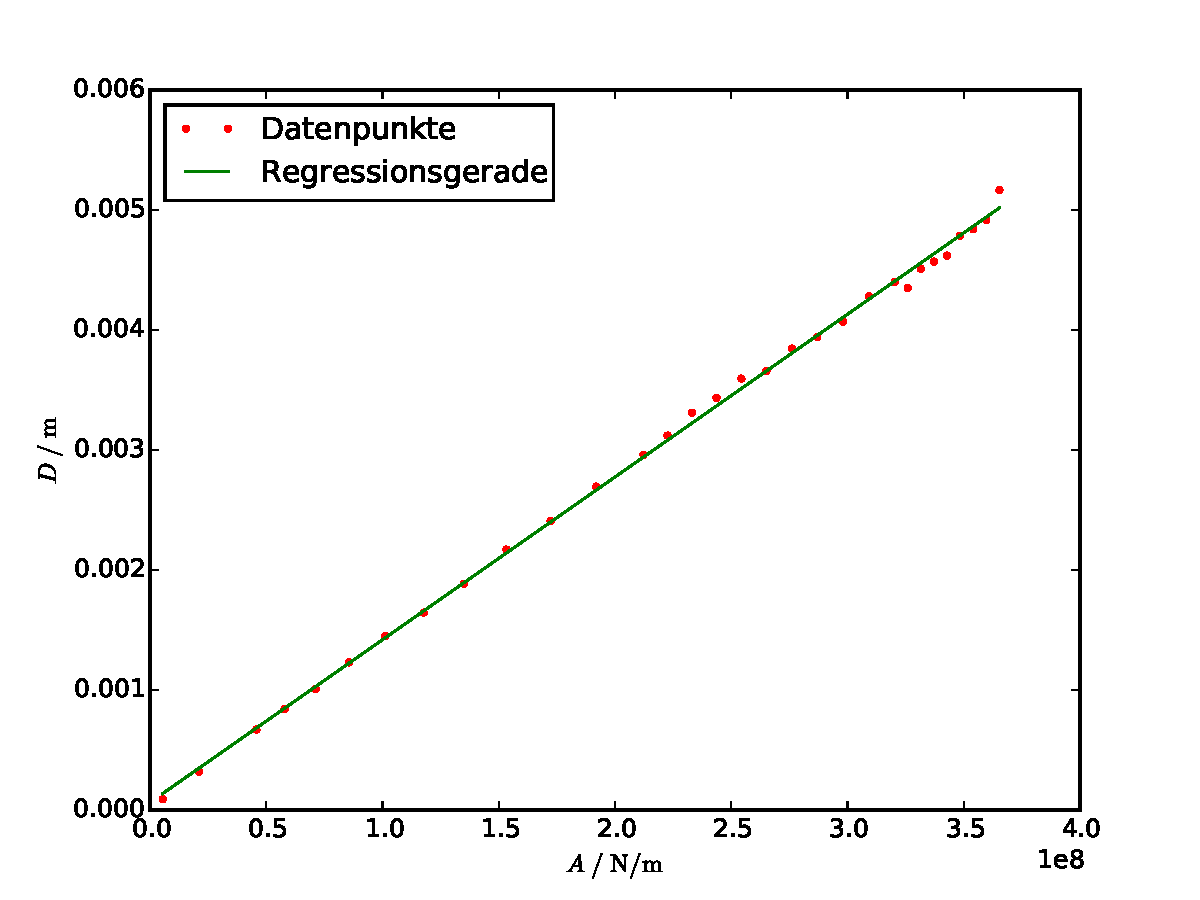
\includegraphics[width=\textwidth]{Regression_eckiger_Stab.pdf}
\caption{Regressionsgerade des eckigen Stabes bei einseitiger Einspannung}
\label{fig:Regression_eckiger_Stab}
\end{figure}







\subsubsection{Eckiger Stab -- beidseitige Einspannung}
Die Bestimmung des Elastizitätsmoduls bei beidseitiger Einspannung ist ähnlich zu der bei einsitiger und unterscheidet sich in der Ausführung im wesentlichen durch die minimal andere Formel \ref{}









\subsection{Bestimmung der Dichte}
Zur Bestimmung der Dichte wurden beide Stäbe , der runde und der eckige, vermessen und gewogen. Das Gewicht und die Länge sind keine fehlerbehafteten Größen. Der Durchmesser hingegen wurde mit einer Schieblehre mehrfach gemessen. Ein Ablesefehler von \SI{0.05}{\milli\metre}  kommt zu dem Fehler des Mittelwertes hinzu.
